\documentclass{acmtog} % V1.2
\usepackage{float}
\usepackage{stfloats}
\usepackage{diagbox}

\acmVolume{}
\acmNumber{}
\acmYear{2019}
\acmMonth{January}
\acmArticleNum{}
\acmdoi{}

\begin{document}

\markboth{V. F. Pamplona et al.}{Photorealistic Models for Pupil Light Reflex and Iridal Pattern Deformation}

\title{Link Prediction in Heterogeneous Networks} % title

\author{Mingze Li {\upshape and} Mingxuan Yan
\affil{Shanghai Jiao Tong University}}

\maketitle
\section{Introduction}
Today, we live in a variety of social networks. It is important and useful for us to figure out an approach to reasonably represent such a social network and make predictions of the relationships inside it. In this project we focus on the work of representation learning in heterogeneous networks, which is the one of the types that the majority of social networks belong to. Its unique challenges come from the existence of multiple types of nodes and links between them, which limit the feasibility of the conventional network embedding techniques. We manage to employ scalable representation learning model called \textbf{metapath2vec++} to overcome the difficulties to embed heterogenous networks. The metapath2vec++ model formalizes meta-path based on random walks in the network to construct the heterogeneous neighborhood of a node and then leverages a heterogeneous skip-gram model to perform node embeddings. The model further enables the simultaneous modeling of structural and semantic correlations in heterogenous networks, which allows us to take advantage of them and make the prediction of the relationships.

\section{Background \& Related Works}
\subsection{Heterogeneous Networks and Social Networks}
According to the original definition, a heterogeneous network is a network that connects computers and other devices with different operating systems and/or protocols\cite{wikipedia}. For instance, the Internet is a heterogeneous network. This is the definition of heterogenous network in the field of communication. While in this project, we consider a heterogeneous network, also can be called heterogeneous information network, as a graph structure that contains different types of nodes, and they are all linked for some certain relationships.
\par In this project, we mainly focus on the research of the relationship in \textbf{Social Networks}, which is considered as heterogeneous networks. A social network is a social structure made up of a set of social actors (such as individuals or organizations), sets of dyadic ties, and social interactions between actors\cite{wikipediasn}. The social network perspective provides a set of methods for analyzing the structure of whole social entities as well as a variety of theories explaining the patterns observed in these structures\cite{WS}.The study of these structures uses social network analysis to identify local and global patterns, locate influential entities, and examine network dynamics. There are lots of different types of network structures in social networks. Here we will start our work on academic conference networks.
\par Here is a diagram of a academic conference network (Fig.\ref{1}). It is a conference network of all the authors and keywords the six conferences contains in a year. In this network, we can see three different types of nodes: the author nodes (orange), the keyword nodes (purple) and the conference nodes (green). The nodes are linked if they have some certain connection between them. Since there are different type of nodes, the links here also represents different meaning. For instance, the link between two author nodes means the two author have cooperated with each other on some paper in this year, the link between the author and the keyword nodes represents that the author published papers containing this keyword, and the link between the author node and the conference node and the link between the keyword node and the conference node both show that they are affiliated to the conference they linked to in this year.
\begin{figure}[H]
  \centering
  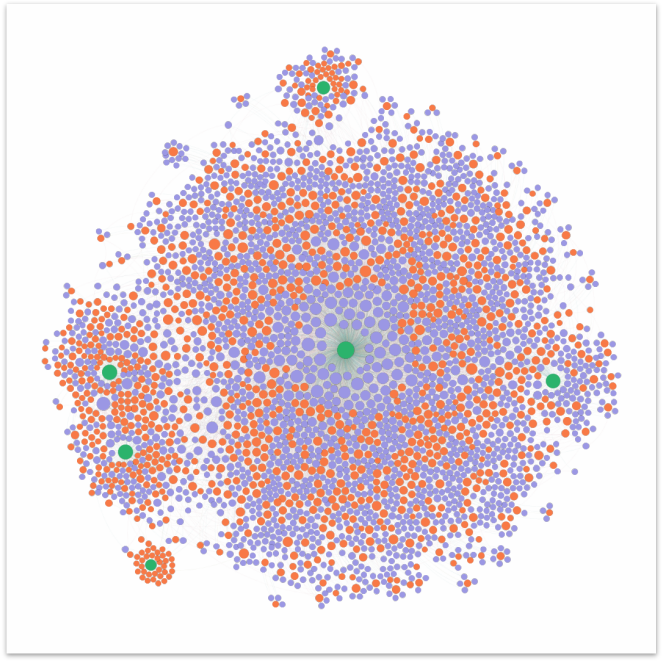
\includegraphics[width=0.7\linewidth]{an.png}
  \caption{Academic conference network}
  \label{1}
\end{figure}
Note that although there are links between different types of nodes, they all represents meaningful relationship that we can employ to form some certain structure. This also suggests that the meaningless relationship does not exist in the network, such as the link between two conference nodes or two keyword nodes. This helps researchers a lot when studying the structure of social networks because the network itself has eliminated many abnormal structures. In this project, it also help us to narrow the expanding choice of meta-path. This part will be explained in details later in the paper.

\subsection{Meta-Path}
A meta-path $P$ is defined in a network structure $T_G = (A, R)$ as a path to link two different type of nodes, which can be formed as:
$$A_1\stackrel{R_1}{\longrightarrow}A_2\stackrel{R_2}{\longrightarrow}\cdots\stackrel{R_i}{\longrightarrow}A_{i+1}$$
where $A_i$ denotes the node type, and $R_i$ denotes the relationship type.
\\By meta-path, a composite relation of two nodes on it can be described as:
$$R = R_1 o R_2 o \cdots o R_i$$
where $o$ is the composition operator of two relations\cite{MP}.
\par In the academic networks, it is very important to form a meta-path structure because it will directly determine the method we explore the network. The following diagram shows examples of meta-path in an academic network.
\begin{figure}[H]
  \centering
  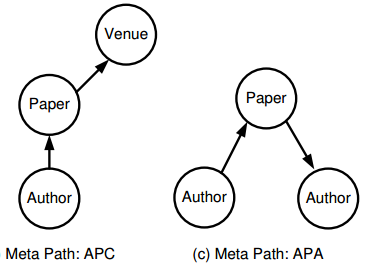
\includegraphics[width=0.7\linewidth]{mp.jpg}
  \caption{Meta-path examples}
  \label{2}
\end{figure}
In this diagram we can see two meta-path: Author $\rightarrow$ Paper $\rightarrow$ Venue $\rightarrow$, and Author $\rightarrow$ Paper $\rightarrow$ Author. These meta-paths will make contribution to the random walks in the network.

\subsection{Random Walk}
A random walk is a mathematical object, known as a stochastic or random process, that describes a path that consists of a succession of random steps on some mathematical space such as the integers\cite{wikipediarw}. Random walks have applications to engineering and many scientific fields including ecology, psychology, computer science, physics, chemistry, biology as well as economics. Random walks explain the observed behaviors of many processes in these fields, and thus serve as a fundamental model for the recorded stochastic activity.
\begin{figure}[H]
  \centering
  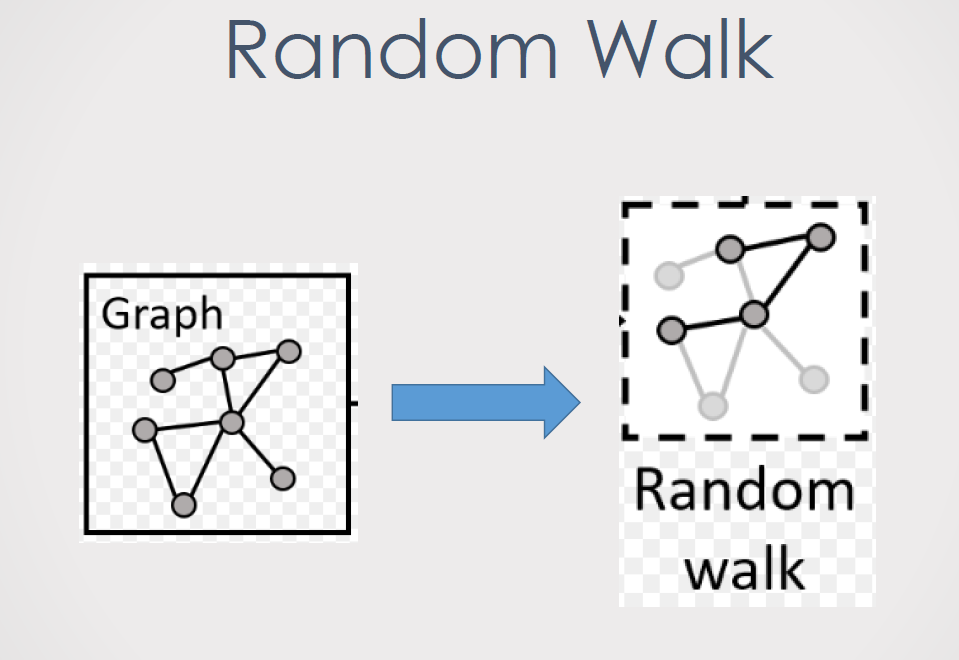
\includegraphics[width=0.7\linewidth]{rw.png}
  \caption{Random walk}
  \label{3}
\end{figure}
\par As shown in Fig.\ref{3}, the random walk process starts from a random node in a graph $G = (V, E)$, and randomly choose the next node from the neighbors to expand to form a random walk path. This is an example of a isomorphic network. If we do random walk procedure in a heterogeneous information network such as a social network, we need to introduce meta-path into random walk, which means that we randomly expand the next node from the neighbors that belong to the certain type of node according to the meta-path.
\par

\subsection{Metapath2vec++}
One of the most important parts of this project is to represent the nodes in the network as vectors, which is also called the vectorization of the network. We form random walk paths in order to provide features for the vectorization procedure.
\par The vectorization method is called \textbf{metapath2vec++}\cite{meta}, which is mentioned in a KDD 2017 research paper: "metapath2vec: Scalable Representation Learning for Heterogeneous Networks". In this paper, the authors provide an algorithm to vectorize the heterogeneous network. The algorithm is shown as follows:
\begin{figure}[H]
  \centering
  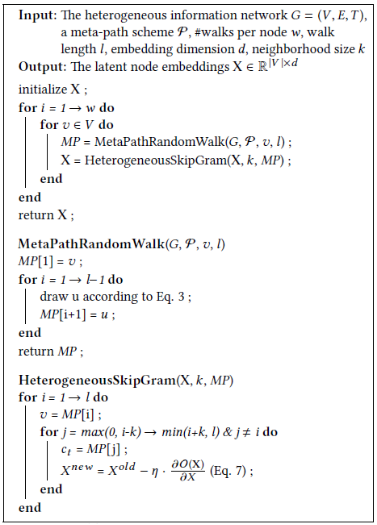
\includegraphics[width=1.0\linewidth]{alg.png}
  \caption{Metapath2vec++ algorithm}
  \label{4}
\end{figure}
\par This metapath2vec++ algorithm also employ some ideas in \textbf{word2vec}, which is proposed by Mikolov et al. to learn the distributed representations of word in natural language\cite{wv}. In the heterogeneous networks, we can regard a random-walk path as a sentence, we employ the skip-gram method to calculate the the similarities in the Time Windows, which can be explained as that centering on one node in the path, and expanding n nodes to the left and the right.
\par With this method, we can execute the vectorization procedure of the academic networks. The detailed work will be explained later in this paper.

\section{Motivation}
The importance of the link prediction in the academic networks is that it will help us better clear a scholar's research direction, find out those other scholars that will cooperate with him or her in the future, make a reasonable prediction of the future development trend of one's research field and estimate the potential conference that the scholar will attend or publish papers on. And also, by this prediction we can estimate the strength of the cooperation between a scholar and his or her coauthors, finding out whether they just temporarily working together or they can form a strong cooperation relationship for a long period of time.
\par Furthermore, if we can get a whole network structure after the prediction process, this structure will further make contribution to the prediction of the research trend of a certain entire field and the leading group of scholars in this field in the future. Currently, researches of using the evolution of the structure of the academic conference networks to make such predictions are not the main stream of the link prediction method, so we would like to attempt to figure out a feasible solution in this direction.

\section{Problem Formulation}
Our problem hypothesis is based on the structure feature of the academic conference network. In this project we will only make the prediction of one year ahead at present. In addition, based on the data set we have got, we are not capable of predict those nodes that has never appeared in the networks before, for example, some new scholars who just step into this field and publish their papers for the first time on these conferences.
\par The main idea of representation of the heterogeneous network is the network vectorization, which means we are going to find a way to represent the different types of nodes in the heterogeneous network with a uniform method -- vectors of the same dimensions. Once we get the vector form of each nodes in the network, the rest of the work is to make the prediction of the relationship between the arbitrary two nodes in the whole structure by calculating the similarity of their vectors.

\section{Proposed Methods}
\subsection{Form random walk paths}
In the previous section, we have introduced random walk method and the reason to form random walk paths based on the meta-path we set previously in a heterogeneous network. In this project, we need to form that random walk paths to vectorize the academic network.
\par The academic network structure we study in this project contains four different types of nodes: Author nodes (A), Keyword Nodes (K), Paper Nodes (P) and Venue nodes (V) (In this project, the academic network we use only contains conferences, so the venue here can also refer to the conference). Here we set the meta-paths to be $AKA$, $AVA$, $AKVKA$ and $AA$. We don't expand the paper node in the meta-path because we find that the paper nodes make the least contribution to mining the hidden relations between author nodes in the network, because the paper nodes just link the authors that has direct connection together, while the keyword nodes can link the authors that may not directly linked to each other together, which is a kind of hidden relations that is not directly shown in the network structure.
\par Then comes to the random walk procedure. In the algorithm, we perform the "random" selection by selecting the nodes with probability. The probability formula the algorithm the employs is shown as follow:
$$ p(v^{i+1}|v^i_t, P) = \left\{
\begin{array}{rcl}
\frac{1}{|N_{t+1}(v^i_t)|}&    &(v^{i+1}, v^i_t) \in E, \phi(v^{i+1}) = t+1\\
0&    &(v^{i+1}, v^i_t) \in E, \phi(v^{i+1}) \neq t+1\\
0&    &(v^{i+1}, v^i_t) \not\in E
\end{array}\right. $$
where $v^i_t$ is a node of the current type $t$, $N_{t+1}(v^i_t)$ denote the number of nodes that linked to the current node of next node type $t+1$ according to the meta-path $P$. $E$ is the edge set of the network. This probability formula indicate that the random walk algorithm only expand the type of nodes that can be linked to the current node type according to the meta-path set previously. The nodes meeting the requirements will be chosen randomly with the same probability, the other nodes will not be chosen to expand, for their probability of 0 calculated by this formula.
\par Meanwhile, we are hoping to introduce the evolution of the network structure through years, since we have got the structures of the same network of different years, so we also allow the random walker to jump to the other year's network with some probability. We considered the whole network as a supernode, and different year's networks are linked in the order of the timeline. We give the random walker a probability of 5\% to jump to the same node in the next network if the next network still has the node in it to conduct cross-level random walk, and the probability of 90\% to stay at the current year's network and conduct the single-level random walk, and also the probability of 5\% to jump back to the previous network.
\par The detailed procedure of random walk can be described as that we do this random walk for each node in the network except all the paper nodes, and we set a length for the random walker to control the length of the path. After the walking, we can use the paths we get to perform the vectorization.

\subsection{Vectorization}
In this part we are going to introduce the detailed vectorization method of the network.
\begin{figure*}[ht]
  \centering
  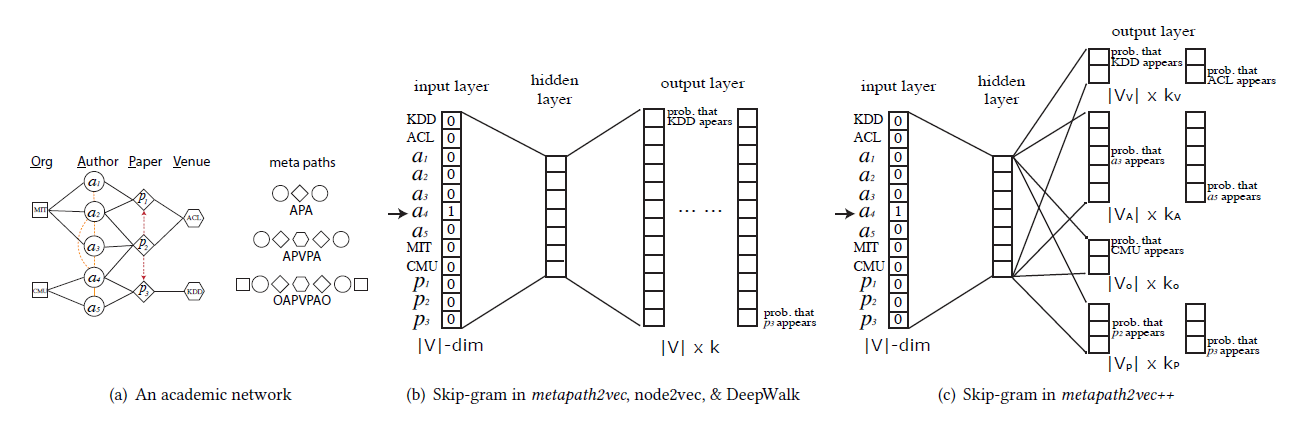
\includegraphics[width=1\linewidth]{ve.png}
  \caption{Vectorization example}
  \label{5}
\end{figure*}
\par In Fig.\ref{5} there are three subfigures indicating the procedures of vectorization. In subfigure (a), there are four types of nodes in the example network, which are author node, paper node, venue node and organization node. The yellow dotted lines in the network denote the coauthor relations and the red dotted lines denote the citation relations. We can also find three meta-paths $APA$, $APVPA$ and $OAPVPAO$. The previous work of vectorization of the network is to form the random walk paths, which is explained in the previous section.
\par In the second subfigure (b), the method \textbf{metapath2vec} is shown. In this graph we take the node $a_4$ as an example to generate the vector representation of this node. We put all the nodes in the random walk path into the model, here it is a $|V|$-dimensional vector where $|V| = 12$ denote the number of the nodes that contains in the random walk path, and $k = 8$ is the number of nodes in the random walk path that can be the neighbors of the goal node $a_4$ in the random walk path. Through the hidden layer, the random walk path will become the vectorization of the target node $a_4$.
\par However, the metapath2vec method only works for the isomorphic network, which means the previous example regard all the nodes in the path as the same type. So in the subfigure (c), the new updated method
\textbf{metapath2vec++} is shown. The difference between metapath2vec and metapath2vec++ is that in the metapath2vec++ method the hidden layer part of the model separately calculate different types of nodes that can be the neighbors to the target node $a_4$. So here the value $k$ has changed to:
$$k = k_V + k_A + k_O + k_P$$
where $k_t$ denotes the number of the neighbor nodes of type $t$.
\par Through metapath2vec++ method we can get a 128-dimensional vector for each node, which we can use for the further calculating of two node vectors' similarity. (Here the number of dimension can be set manually)

\section{Experiments}
In this project, the data we use is the information of the authors, papers and the keywords of 5 conferences: MOBICOM, INFOCOM, SIGCOMM, ISDA and OSDI in year 2011, 2012, 2013 and 2014. We use these information to form the academic network first and generate the random walk paths and vectorization the networks first. Since we introduce cross-level random walk into the project, so we use the random walker to walk through the networks of year 2011, 2012 and 2013 to make the prediction of the relations in year 2014, then use the prediction to compare with the actual structure of the network of year 2014 to test the reliability of our prediction method.
\par After we get the vector representations of the nodes in the networks, we calculate the similarity of two vectors to estimate the relation of the two corresponding nodes. The method we use in this project to calculate the similarity is to calculate the Euclidean distance of the two vectors. The smaller the distance is, the more similar the two vectors are, and the relation between the two node is more strong.
\par To test the accuracy of the algorithm, we estimate the relations of 10000 authors in the network, predict the top 10 nodes with the strongest relation with the node if it has more than 10 adjacent nodes and compared with the neighboring nodes in the actual network of year 2014. The testing result is shown as follows:
\begin{table}[H]
  \centering
  \begin{tabular}{|c|c|c|c|}
    \hline
    \diagbox{meta path}{Node type}&$A$&$K$&$V$\\
    \hline
    $AKA$ $AKVKA$ $AA$&78.563\%&not accurate& not accurate\\
    \hline
    $AKA$ $AVA$ $AA$&82.343\%&not accurate&not accurate\\
    \hline
  \end{tabular}
\end{table}
Note: in the testing result table above, the "not accurate" means that the prediction accuracy of that type of node is less than 50\% and fluctuate wildly every time we run the program.

\section{Conclusion}
From the result get from the experiment shown in the previous section, we found that the accuracy of the relation prediction of the author nodes meet our expectation. However, the result keyword nodes and the venue nodes (Conference nodes) are not that stable and accurate. We think the reason that the result of keyword nodes and the venue nodes are not very good is that they are not the same type with the author node, so the similarity estimation will not be that accurate.
\par The result shown in the previous section is based on the random walk path with the length of 100. Since the length of random walk path can be manually tuned, we also run the result of different length of random walk path to see the result. The result is shown as follows:
\begin{table}[H]
  \centering
  \begin{tabular}{|c|c|c|c|}
    \hline
    \diagbox{path length}{Node type}&$A$&$K$&$V$\\
    \hline
    100&83.152\%&not accurate& not accurate\\
    \hline
    1000&86.273\%&72.438\%&79.713\%\\
    \hline
  \end{tabular}
\end{table}
\par From this table we see that with the increase of the length of random walk path, the prediction results of the keyword nodes and the venue nodes have been stable and met our expectation. So we conclude that prediction of the relations between different type of nodes requires longer random walk path than the prediction of the relation between the nodes of the same type.
\par Through the experiment, we find that the vectorization of the heterogeneous network can actually help us unify the structure of the network and find the hidden relations in it that are not directly shown by links. The hidden relations here actually means that if we find the two authors are linked to each other in the actual structure while we predict them to be unlinked, so they just cooperate with some work in this year, but they are not going to have a long-term cooperation in the future because based on our prediction, their vectors are not that similar, which means that the other nodes that link to them varies a lot; but if we find two authors do not link to each other in the real structure but we predict them to be linked, the situation is totally opposite, they may work in the same field and will form a cooperation relationship in the future. And trough the result, we found that our method has reached a relatively accurate state. So in the future, we will continue to improve the accuracy of our method to utilize this method into the relation prediction in the heterogenous networks and other related work such as the prediction of a scholar's academic career.

\section*{Acknowledgements}
In this semester we are very honored to have the algorithm design course by Professor Jiang. Algorithm design is the basement subject of computer science, and Professor Jiang helps us build a very solid foundation for our future study and research. Here we are also very thankful for the help given by Professor Jiang and the tutors during the class and the project. We sincerely wish that this course will be better and better.


% Bibliography
\bibliographystyle{ACM-Reference-Format-Journals}
\bibliography{acmtog-sample-bibfile}





\end{document}
